\documentclass[fleqn,10pt]{olplainarticle}
\usepackage{hyperref}

\usepackage{xcolor}
\hypersetup{
	colorlinks,
	linkcolor={red!50!black},
	citecolor={blue!50!black},
	urlcolor={blue!80!black}
}

\usepackage{enumitem}

\usepackage{float}

\usepackage{caption}
\usepackage{subcaption}
\usepackage{multicol}

\usepackage{lscape}
\usepackage{makecell}

\usepackage{color}
\usepackage{colortbl}



% Use option lineno for line numbers 

\title{Cross-chain Secure Messaging}

\author[1]{jistro.eth~~~~0xVato.stark~~~~ariutokintumi.eth}
%\author[2]{Ariutokintumi.eth }
%\affil[1]{Address of first author}
%\affil[2]{Address of second author}

\keywords{Cross-chain, Blockchain}


\begin{abstract}
In this study, we explored solutions, and challenges in cross-chain implementations, providing a glimpse into the strengths and limitations of different of cross-chain solutions.
\end{abstract}

\begin{document}

\flushbottom
\maketitle
\thispagestyle{empty}

\tableofcontents

\section{Cross-chain Solutions}

\subsection{Axelar}

In the case of Axelar, we reference the documentation for calling a contract on chains \cite{axelar_axelar_nodate}. The sender employs the \texttt{gateway.callContract} command, specifying the message, \texttt{destinationChain} (a string indicating the chain name), \texttt{destinationAddress} (a string denoting the Smart Contract address of the receiver), and the value in the local token of the chain, covering the transaction cost within Axelar.

The corresponding code can be analyzed and utilized from the following link: \url{https://github.com/Roll-a-Mate/Research/blob/main/0003-CrossChainSecureMessaging/Code/Axelar.sol}

Upon sending the message in this instance, from Ethereum on the Sepolia chain with the contract address \texttt{0x490c2aD342C42fb60148d57cAEEB6Cbc1521685b} to Polygon Mumbai using the contract address \texttt{0x81a1e2DDa1aE7DFA35631075898ee72D30965370}, obtaining the transaction hash is crucial for monitoring the process (see Figure \ref{fig:axelartxseptomum}). The entire duration of this transaction is 16 minutes and 50 seconds, incurring a cost of 0.000509 ETH, equivalent to 1.12 USD (as of January 3, 2024).


Unfortunately, the interaction from Polygon Mumbai to Ethereum Sepolia failed due to the higher base fee, approximately 6 Matic tokens (as of January 3, 2024), resulting in the message not being sent (see Figure \ref{fig:axelartxmumtosepfail}).

\begin{figure}[!h]
	\begin{subfigure}{.5\textwidth}
		\centering
		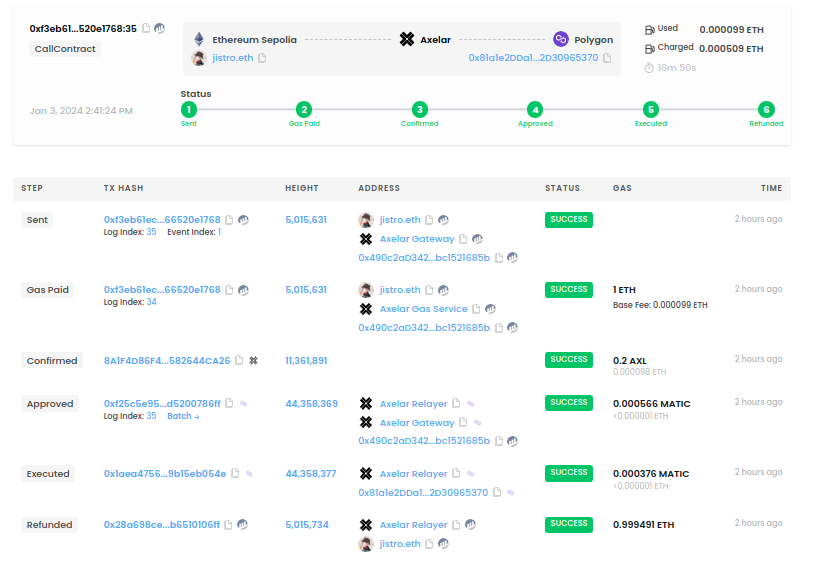
\includegraphics[width=1\linewidth]{img/AxelarTxSepToMum}
		\caption{Transaction from Ethereum Sepolia to Polygon Mumbai}
		\label{fig:axelartxseptomum}
	\end{subfigure}
	\begin{subfigure}{.5\textwidth}
		\centering
		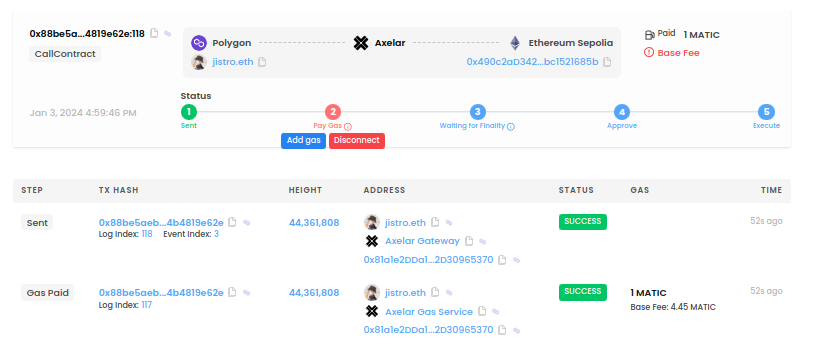
\includegraphics[width=1\linewidth]{img/AxelarTxMumToSepFail}
		\caption{Failed Transaction from Polygon Mumbai to Ethereum Sepolia}
		\label{fig:axelartxmumtosepfail}
	\end{subfigure}
	\caption{Axelar Transactions}
	\label{fig:inputIMG}
\end{figure}

Axelar has the most straightforward and developer-friendly implementation. However, concerns arise about the security using strings for \texttt{destinationChain} and \texttt{destinationAddress}, and the volatile base fee for chains that do not have ETH as their main token, making cost estimation a bit challenging.

\newpage

\subsection{Hyperlane Implementation}

During the implementation of Hyperlane, we encountered challenges with the smart contract integration. The documentation proved to be confusing and, in some instances, contained errors. Consequently, developers spent additional time investigating a task that could have been completed more efficiently.

Once the challenges were overcome in the implementation phase, we created a Smart Contract on Ethereum Sepolia with the address \texttt{0xECBc8094DebB430d5E75afCAFe6a18422f73BF32}. This Smart Contract is designed to make a call to a receiver contract in Polygon Mumbai with the Smart Contract Address \texttt{0x69D69632dfC69C1714CED0CE2CE6F15285da6478}.

The corresponding code can be analyzed and utilized from the following link:
\url{https://github.com/Roll-a-Mate/Research/blob/main/0003-CrossChainSecureMessaging/Code/Hyperlane.sol}

Using the transaction hash in the explorer provides the result of the Cross-Chain call process, taking 57 seconds. Unfortunately, the explorer does not provide the transaction cost in ETH for the transaction (see Figure \ref{fig:hyperlaneethtomum}).

\begin{figure}[h]
	\centering
	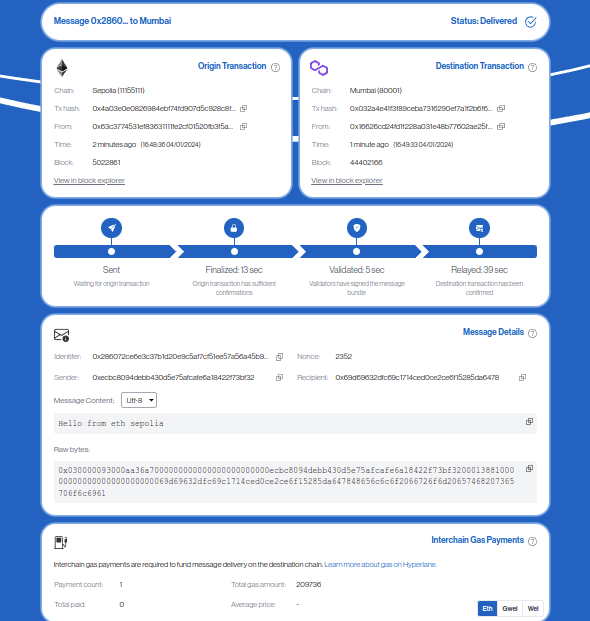
\includegraphics[width=0.7\linewidth]{img/HyperlaneEthToMum}
	\caption{Transaction Result for Hyperlane Cross-Chain Call}
	\label{fig:hyperlaneethtomum}
\end{figure}

While seeking assistance in the official Discord channel, the team and I discovered some bugs in the documentation, particularly regarding the \texttt{IMailbox} smart contract invocation. There were misspelled variables for the \texttt{dispatch} function. Hyperlane assured us that they intend to improve this documentation as soon as possible.

The lack of comprehensive documentation and absence of pricing information on the explorer for Hyperlane posed significant challenges during implementation. The investment of additional time was necessary to ensure a correct and efficient integration process.


\subsection{Chainlink CCIP}

Utilizing the documentation for sending arbitrary data \cite{noauthor_CCIP_nodate}, the sender employs the \texttt{outer.ccipSend} function. This function facilitates the transmission of a message, requiring parameters such as \\ \texttt{destinationChainSelector} (a uint64 indicating the chain location), \texttt{\_receiver} (an address value denoting the Smart Contract address of the receiver), and the fee, which can be covered in LINK tokens or the native chain token.

The corresponding code can be analyzed and utilized from the following link:
\url{https://github.com/Roll-a-Mate/Research/blob/main/0003-CrossChainSecureMessaging/Code/CCIP.sol}

Executing this operation from the contract \\ \texttt{0x76c9b90A6c62c24FA711d4aF123D8FA3f52D6c58} in Ethereum Sepolia with a deposit of 5 LINK tokens to the contract, the message is sent to Polygon Mumbai using the contract address \texttt{0xa810b54E2c5c89Db6069Bc14613Af86586142aE7}. In Axelar, the transaction hash plays a crucial role in obtaining cross-chain transaction details. The entire duration of this transaction (see Figure \ref{fig:ccipethseptomum}) is 21 minutes, incurring a cost of 0.045014064168071695 LINK, equivalent to 0.64 USD (as of January 3, 2024).
 

\begin{figure}[H]
	\centering
	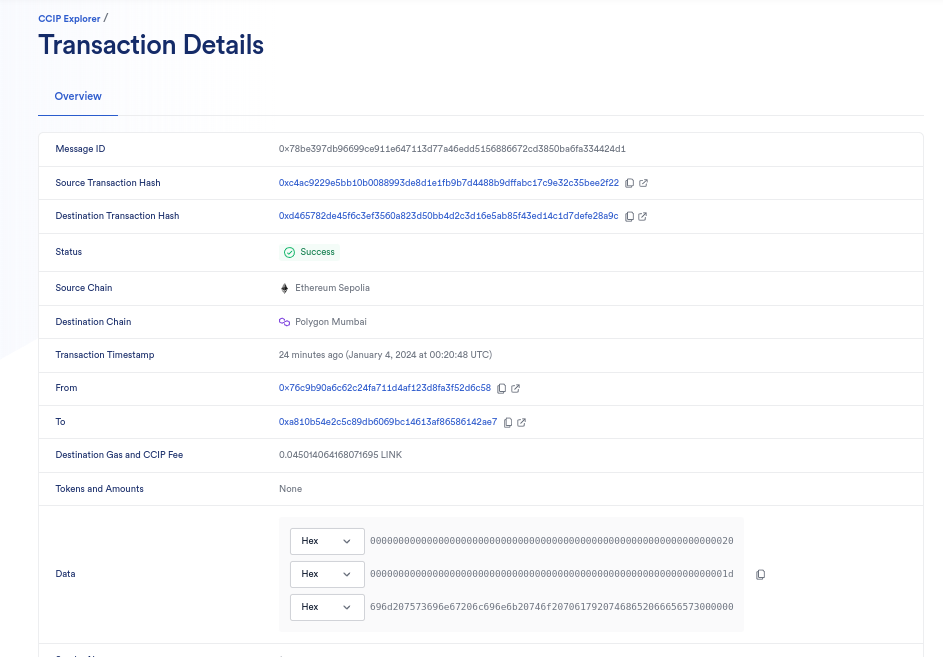
\includegraphics[width=.6\linewidth]{img/CcipEthSepToMum}
	\caption{CCIP transaction}
	\label{fig:ccipethseptomum}
\end{figure}


Chainlink's CCIP brings a similar experience to Axelar, but the price can be stable if we use the LINK token as a transaction fee. The problem with this solution is the time required for validation from Ethereum to any chain, which is significantly slower compared to other solutions.


\section{Layer Zero}

Based on the documentation from Layer Zero Getting Started \cite{layer_zero_Getting}, we first defined the endpoint address and the endpoint id. An interesting aspect of the endpoint (especially for the testnet chains) is that almost all chains share the same address, providing a seamless developer experience where every number corresponds to a uint32.

For this implementation, we deployed a smart contract for the Ethereum Sepolia testnet with the address \texttt{0x3E6a9bFA458242b6E123700244485169a31E48B7} as the sender. The smart contract receiver is deployed on the Optimism testnet with the address \\ \texttt{0x58B5baB0a2df888501b8bC4CEF2391Df002674A5}. This choice is made because the Message Execution Options are optimized for messages sent to the Optimism testnet. Citing the LayerZero documentation for Message Execution Options \cite{layer_zero_options}:

\begin{quote}
	"LayerZero provides robust Message Execution Options, allowing you to specify arbitrary logic as part of the message transaction, such as the gas amount and \texttt{msg.value} the Executor pays for message delivery, the order of message execution, or dropping an amount of gas to a destination address."
\end{quote}

The corresponding code can be analyzed and utilized from the following link:
\url{https://github.com/Roll-a-Mate/Research/blob/main/0003-CrossChainSecureMessaging/Code/LayerZero}

When executing the sender contract using 1 ETH for testing the Layer Zero refund function, the entire duration of this transaction (see Figure \ref{fig:layerzeroethtoop}) was 25 seconds. We incurred a cost of 200,000 Wei (0.0000000000002 ETH), which, as of the writing of this section (January 12, 2024), is equivalent to 0.00000000051 USD.

\begin{figure}[H]
	\centering
	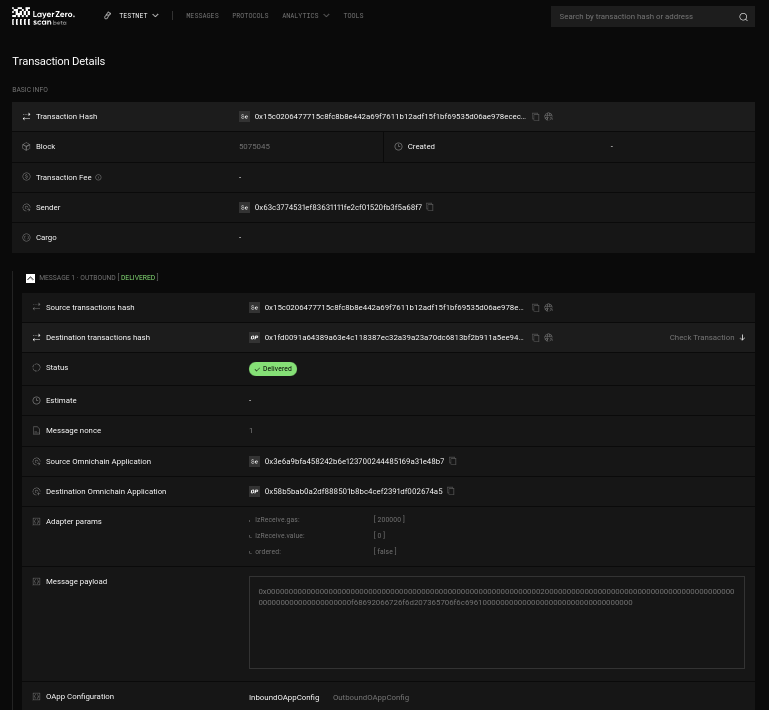
\includegraphics[width=0.7\linewidth]{img/LayerZeroEthToOP}
	\caption{Layer Zero ETH to Optimism Transaction}
	\label{fig:layerzeroethtoop}
\end{figure}


Layer Zero provides a permissionless protocol for sending messages chain to chain. However, as observed in Hyperlane and Axelar, the transaction cost for every transaction can be volatile because Layer Zero uses the main token as the transaction cost.





\begin{table}[H]
	\tiny
	\centering
	\begin{tabular}{|c|c|c|c|c|c|}
		\hline
		Solution  
		& \makecell{Delay\\ Ethereum $\longrightarrow$ Polygon}  
		& \makecell{Delay\\ Polygon $\longrightarrow$ Ethereum}
		& \makecell{Cost per Message\\ Ethereum $\longrightarrow$ Polygon}  
		& \makecell{Cost per Message\\ Polygon $\longrightarrow$ Ethereum}  
		& Consensus         \\ \hline
		
		Axelar    
		& 18m 52s \cite{noauthor_interchaintransfer_ETH_MATIC}                       
		& 16m 39s  \cite{noauthor_interchaintransfer_MATIC_ETH}         
		& 0.000595 ETH \cite{noauthor_interchaintransfer_ETH_MATIC}                  
		& 12.17 MATIC  \cite{noauthor_interchaintransfer_MATIC_ETH}             
		& Proof of stake nodes \\ \hline
		
		Hyperlane 
		& 3m 3s \cite{noauthor_hyperlane_ETH_MATIC}                     
		& 10m 20s \cite{noauthor_hyperlane_MATIC_ETH}    
		& 0.00002339021594448 ETH  \cite{noauthor_hyperlane_ETH_MATIC}           
		& 20.380072606431995 MATIC  \cite{noauthor_hyperlane_MATIC_ETH}            
		& Per-origin-chain \cite{hyperlane_validators_nodate}    \\ \hline
		
		CCIP      
		& 25m 46s \cite{ccip_ETH_MATIC}                          
		& 3m 6s\cite{ccip_MATIC_ETH}       
		& 0.008620804720114726 LINK \cite{ccip_ETH_MATIC}   
		& 2.534953023940595 LINK \cite{ccip_MATIC_ETH}
		& Chainlink Oracles \cite{chainlink_ccip_nodate} \\ \hline
		
		Layer Zero 
		& 3m 46s \cite{LZ_ETH_MATIC}                        
		& 20m 40s \cite{LZ_MATIC_ETH}    
		& 0.000352500782360452 ETH \cite{LZ_ETH_MATIC}          
		& 0.006596250005936625 MATIC \cite{LZ_MATIC_ETH}             
		& Oracles \cite{obasi_layerzero_2023}    \\ \hline
	\end{tabular}
	\caption{Comparative Cross-Chain Solutions Data using Ethereum and Polygon.}
	\label{tab:TableCrossChain}
\end{table}



\newpage
\bibliography{citations}

\end{document}